\documentclass{article}
\usepackage[usenames,dvipsnames]{color} % Required for custom colors
\usepackage{graphicx} % Required to insert images
\usepackage{listings} % Required for insertion of code
\usepackage{amsmath} % Required for some math formulas
\usepackage{enumitem} % Required for customed enum
\usepackage{url} % Auto line break in URL
%\usepackage{tabularx} % Auto line break in tabular
\usepackage{ltablex} % Required for auto page break tabular
\usepackage{booktabs} % Required for table
\usepackage{dirtree} % Required for directory tree
\usepackage{verbatim} % Required for typesetting diff 
\makeatletter

\long\def\diffcolor#1#2\@nil{color\string#1diff}

\def\verbatim@processline{%
\nointerlineskip\noindent\rlap{%
\colorbox{\expandafter\diffcolor\next..\@nil}{%
\the\verbatim@line}}\par}
\makeatother

\definecolor{color diff}{rgb}{1,1,1}
\definecolor{color-diff}{rgb}{1,.5,.5}
\definecolor{color+diff}{rgb}{.5,1,.5}

\def\UrlBreaks{\do\[\do\\\do\]\do\^\do\_\do\`\do\.\do\@\do\\\do\/\do\!\do\_\do\|\do\;\do\>\do\]\do\)\do\,\do\?\do\'\do+\do\=\do\#}

\usepackage{hyperref} % add clickable link to contents
\hypersetup {
    colorlinks = false, % links colored or not
    hidelinks = true, % border
    linkcolor = blue, % color TOC links in blue
    urlcolor = red, % color URLs in red
    linktoc = all % 'all' will create links for everything in the TOC
}

% Uncomment the lines below if you wish to use Chinese characters
\usepackage{fontspec}  % Chinese characters support
\usepackage{indentfirst} % Add indent at the first paragraph
\XeTeXlinebreaklocale "zh" % Automatic line break
\XeTeXlinebreakskip = 0pt plus 1pt % Automatic line break
% \setmainfont{STSong} % Use a Chinese font
% \setmainfont[Path = ./]{AdobeSongStd-Light.otf} % use font in ./
\setmainfont[Path = fonts/]{AdobeFangsongStd-Regular.otf}

% Use Chinese for figure name
\renewcommand\figurename{图}

% Use Chinese for contents name
\renewcommand\contentsname{目录}

% Use Chinese for table name
\renewcommand\tablename{表}

% contents depth
\setcounter{tocdepth}{4}

% numbered paragraph
\setcounter{secnumdepth}{4}

%----------------------------------------------------------------------------------------
%	TITLE SECTION
%----------------------------------------------------------------------------------------

\newcommand{\horrule}[1]{\rule{\linewidth}{#1}} % Create horizontal rule command with 1 argument of height

\title{	
\normalfont \normalsize 
% \textsc{university, school or department name} \\ [25pt] % Your university, school and/or department name(s)
\horrule{0.5pt} \\[0.4cm] % Thin top horizontal rule
\huge Cache Debugger使用手册 \\ % The assignment title
\horrule{2pt} \\[0.5cm] % Thick bottom horizontal rule
}

\author{Cache小组} % Your name

\date{\normalsize\the\year 年\the\month 月\the\day 日} % Today's date or a custom date




% document begin
\begin{document}
\maketitle % Print the title

\tableofcontents % Print the contents

\newpage % blank after contents

\section{引言}
    \subsection{开发信息}
        系统名称:硬件调试工具Cache Debugger

        开发者:
        \begin{minipage}[t]{0.8\linewidth}
        计23 李天润

        计23 胡津铭

        计23 孙皓
        \end{minipage}

    \subsection{内容简介}
        本文档介绍了硬件调试工具的功能设计以及软硬件部分实现细节,方便读者更深入了解本工具的运行方式,以及根据自己的需要对工具进行修改、开发。

        本文档假设读者已经阅读过调试工具的使用手册,并且了解硬件描述语言的基本应用以及元件例化的方法。

\section{设计原理}
    硬件逻辑分时序逻辑与组合逻辑,其中组合逻辑仅与输入有关,时序逻辑受时钟控制。

    在系内课程与FPGA有关的实验中,并没有涉及与延时相关的逻辑,比如振荡电路,因此FPGA芯片内部的硬件延时在设计硬件逻辑时一般不会被考虑,仅影响时钟频率的提高。%
    基于以上考虑,可以认为大多数实验中,硬件逻辑的执行是由时钟驱动的,因此控制了时钟也就控制了逻辑的执行。%
    而且,由于设计逻辑时不会将延时作为正面的逻辑功能的一部分,时钟沿无论延迟多久到达都不会产生负面作用,因此暂停时钟相当于将电路暂停,之后再次给入时钟信号即可无损地继续执行程序。

    本工具正是基于以上结论,结合调试的断点信息,产生被调试模块的时钟信号,使得被调试模块既可正常运行,又可以在给定的状态下暂停,查看调试信息。

    通过逻辑操作,本工具可以为被调试模块提供与调试工具的输入时钟信号相同频率的时钟信号,使得被调试模块在调试环境下有着与实际单独运行时几乎相同的表现。

\section{概述}
    \subsection{用途}
        Cache Debugger是一个基于串口的VHDL通用调试工具。%
        使用本工具可以在PC端发送指令到硬件系统,%
        具有启动、断点、继续运行、单步调试、查看信号等多种功能。%

    \subsection{系统配置}
        带有串口的目标设备
        
        支持VHDL语言和该目标设备的集成软件开发环境

        Unix或类Unix操作系统,安装有串口设备驱动,支持C++11的编译器

    

\section{硬件部署}
    以一个简单的计时器为例叙述如何将本工具应用于被测试模块。

    首先在被测试模块的实体中加入两个输出信号:被查看信号和断点条件。

    在结构体的并发处理语句中定义被查看信号和断点条件。%
    被查看信号的定义可使用工具自动生成,默认8对齐,未使用的用0填充。%
    断点条件未使用的部分必须用0填充。

    在本例中被查看信号共4096位,断点条件64位。%
    被查看的信号microsecond类型为std\_logic\_vector,共10位,%
    用0填充6位以实现8对齐。%
    被查看的信号millisecond类型为std\_logic\_vector,共10位,%
    用0填充6位以实现8对齐。%
    断点条件分别为second、millisecond、microsecond。

    \verbatiminput{diff/debugged.diff}
    
    在新的顶层模块中原件例化被调试的模块,并将输出端口对应起来。

    \verbatiminput{diff/cadb.diff}

    将50MHz时钟连接到bp\_debug模块的输入时钟,%
    将bp\_debug模块的输出时钟连接到被调试模块的时钟。

    为cadb分配串口管脚。

\section{软件部署}
    首先编写配置文件,配置文件共三列。

    第一列是软件端查看变量值时的标签,接受不包含空白字符的字符串。

    第二列是VHDL源代码中实际被查看信号名称,%
    接收不包含空白字符的字符串,在被调试模块中应有同名信号,%
    且该信号不能为输出端口。

    第三列是被查看信号的范围。%
    对于std\_logic\_vector应标明范围,%
    对于std\_logic第三列空。

    配置文件支持\#风格的注释。

    运行软件端程序cadb gen <目标文件>,%
    信号定义部分VHDL代码将自动生成并保存在目标文件中。

    每次更新配置文件后都应该重新生成VHDL代码并将其更新到硬件中。

    运行cadb <串口设备路径>,调试工具将启动。


\section{使用方法}
    软件端程序启动后应该出现如图\ref{client}所示界面,此时输入命令help可查看帮助。

    \begin{figure}[!hbp]
            \caption{软件端界面}\label{client}
            \centering
            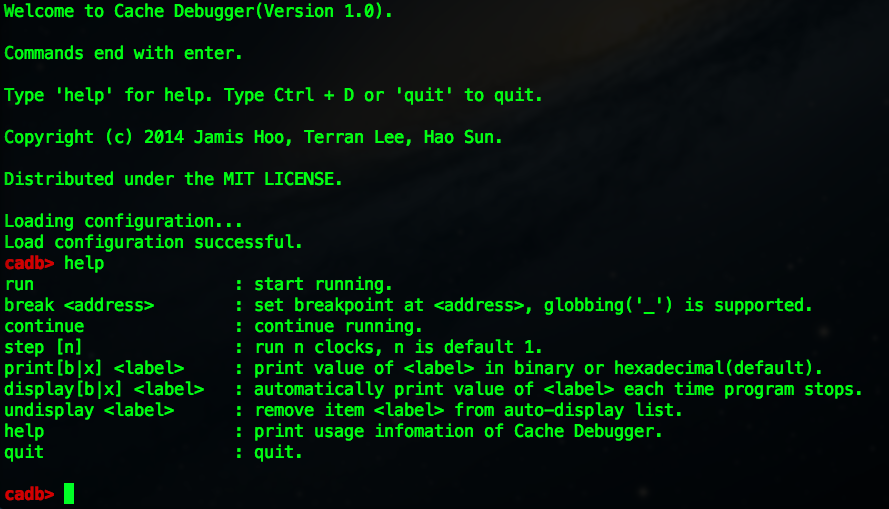
\includegraphics[width=\textwidth]{chart/cadb_client}
    \end{figure}

    所有支持的命令:
    \begin{enumerate}
    \item
    run: 开始运行。
    \item
    break <value>: 设置断点,支持十六进制(0x)和二进制(0b)。
    \item
    continue: 继续运行。
    \item
    step [n]: 前进n个时钟,n默认为1,支持二进制、八进制、十进制、十六进制。
    \item
    print[b|x] <label>: 以二进制(b)或十六进制打印变量。默认为十六进制。
    \item
    display[b|x] <label>: 自动打印变量。
    \item
    undisplay <label>: 取消所有该变量的自动打印。
    \item
    help: 显示帮助信息。
    \item
    quit: 退出。
    \end{enumerate}

    输入run相当于被调试模块得到一个reset信号后得到连续的时钟信号,%
    被调试模块应该在此条件下能正确运行。

    输入run、step、continue命令后程序会阻塞,%
    直到到达断点条件,用户才可继续操作,此时可使用print命令查看信号值。

    断点设置有高级用法,参见技术文档。


\section{维护}
    如果在使用中遇到问题请仔细阅读使用手册和技术文档,%
    确保使用方法正确,满足设计约定。%
    如果问题仍然不能解决,请联系作者,联系方式请咨询本使用手册提供者。


\end{document}
